\textit{Cette partie présente \emph{Hibernate}, l'ORM que nous avons du utiliser pour gérer l'accès aux données. Elle détaille également les différents packages de l'application, la manière dont ont été mappé les informations, la manière adoptée pour la génération du graphe, ainsi que l'utilisation de l'outil développé en ligne de commande. Notons que l'utilisation du langage Java ne sera pas justifié étant donné qu'il s'agit d'une contrainte induite pas le fait que le framework \emph{Hibernate} devait être utilisé.}

\section{L'ORM \emph{Hibernate}}
Hibernate est un framework Java de type ORM. Bien qu'il permette la gestion de la persistance des données (écriture), Hibernate sera utilisé ici uniquement dans le but d'accéder aux métadonnées des SGBD (lecture) via des configurations de Mapping.
\subsection{POJO}
La définition des entités dans \emph{Hibernate} à l'aide de classes \emph{POJO}. Cet acronyme signifiant \og Plain Old Java Object \fg{} fait référence à de simples classes ayant comme principale caractéristique de n'implémenter aucune interface, et de posséder un \emph{getter} et un \emph{setter} par attribut.
\subsection{Mapping}
Le mapping consiste, comme son nom l'indique, à faire la liaison entre les entités définies (classes \emph{POJO}) et les tables en base de données. En règle générale, un objet $x$ est mappé avec une table relationnelle $table-x$, est les attributs $x_1$, $x_2$, \ldots, $x_n$ avec les attributs $tables-x.x_1$, $tables-x.x_1$, \ldots, $tables-x.x_1$. Il est également possible d'ajouter des relations entre attributs (One-to-One, One-to-Many, Many-to-Many), de déclarer des \emph{id}, etc.

\emph{Hibernate} permet de définir le mapping via des annotations directement au sein des classes, ou via des fichiers de configuration xml \texttt{hbm}. C'est cette deuxième méthode que nous avons choisie, et qui sera décrite dans la partie~\ref{section:structure_de_lapplication}.
\subsection{Subselect}

\subparagraph{\ldots}

\section{Structure de l'application}
\label{section:structure_de_lapplication}

Dans le but de faciliter la réutilisation du code et l'extension de sa compatibilité avec de nouveaux SGBD, nous avons pris soin de structurer l'application. La figure~\ref{figure:structure_appli} présente l'arborescence des paquets Java.

\begin{figure}[H]
\centering
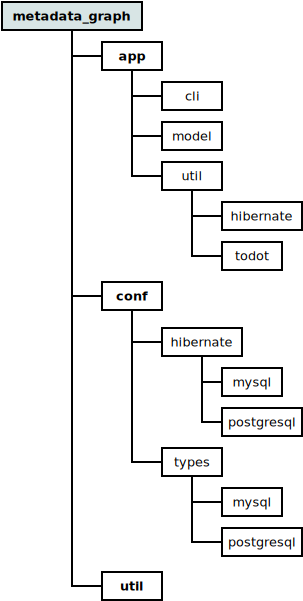
\includegraphics[width=0.5\textwidth]{files/archi}
\caption{Arborescence des paquets Java de l'application.}
\label{figure:structure_appli}
\end{figure}

Trois paquets principaux se distinguent :

\begin{description}
\item[\texttt{app}] : dans ce paquet sont regroupé toutes les classes Java nécessaires au fonctionnement interne de l'outil. On y trouve les sous paquets \texttt{cli}, \texttt{model} et \texttt{util} qui seront détaillés par la suite.
\item[\texttt{conf}] : ce paquet permet d'externaliser les fichiers de configuration. Il a la particularité de ne stocker aucune classe Java.
\item[\texttt{util}] : ici sont regroupés des classes java utilisés par l'application mais qui ne sont pas propre à l’exécution de ses fonctions initiales. Elle stocke notament des classes permettant la gestion du CLI.
\end{description}

\subsection{Paquet \texttt{app.cli}}
\subsubsection{Utilisation}

\subsection{Paquet \texttt{app.model}}
C'est ici que sont définies les classes \emph{POJO} du modèle de donnée correspondant au modèle relationnel. On y trouve donc classes \texttt{Column}, \texttt{Constraint} et \texttt{Table}, enrichies de quelques méthodes :

\begin{description}

\item[Column] Ajout d'un méthode \texttt{\underline{bool isPk()}} permettant de savoir si la colonne est inclue dans la clé primaire de la table à laquelle elle appartient. Une méthode \texttt{\underline{String getGenericType()}} qui retourne, sous la forme d'une chaine de caractères, le type générique de la colonne est également définie.

\item[Constraint] Ajout des méthodes \texttt{\underline{bool isPk()}}, \texttt{\underline{bool isFk()}} et \texttt{\underline{bool isCheck()}} permettant de savoir respectivement si la contrainte est de type clé primaire, clé étrangère, ou check. Une méthode \texttt{\underline{String getGenericType()}} qui retourne, sous la forme d'une chaine de caractères, le type générique de la contrainte est également définie.
\end{description}

Les types génériques sont définies dans les énumérations \texttt{ColumnType} et \texttt{ConstraintType}. Les conversions de types se font en fonction du SGBD sélectionné grâce au paquet \texttt{app.util} (cf. \ref{subsection:app.util}) aux fichiers de conversions stockés dans le paquet \texttt{conf.types} (cf. \ref{subsection:conf.types}).

\subsection{Paquet \texttt{app.util}}
\label{subsection:app.util}
\subsubsection{Génération de graphe}

\subsection{Paquet \texttt{conf.hibernate}}
\subsubsection{Fichiers de mapping}
\subsubsection{Subselect}

\subsection{Paquet \texttt{conf.types}}
\label{subsection:conf.types}


\section{Utilisation de \emph{graphviz}}
dot, neato, etc.